\documentclass[11pt, a4paper]{article}

% Pacchetti base per lingua e codifica
\usepackage[utf8]{inputenc}
\usepackage[italian]{babel}

% Pacchetti per la matematica e la fisica
\usepackage{amsmath, amssymb, amsfonts}
\usepackage{cancel} % Utile per sbarrare i termini che si annullano

% Pacchetti per la grafica e l'impaginazione
\usepackage{graphicx}
\usepackage{geometry}
\geometry{top=2.5cm, bottom=2.5cm, left=2.5cm, right=2.5cm}
\usepackage{booktabs}
\usepackage{multirow}
\usepackage{sectsty}
\usepackage{float}
\usepackage{xcolor}
\allsectionsfont{\underline}
\setcounter{secnumdepth}{0}

\begin{document}
\tableofcontents

\newpage

\section{Particella Libera 1D} %

Consideriamo una particella libera di muoversi in una dimensione, senza forze applicate: %
\begin{equation*}
    \boxed{ \hat{V} = 0 } \quad \Rightarrow \quad \hat{H} = -\frac{\hbar^2}{2m} \frac{\partial^2}{\partial x^2} %
\end{equation*}

\noindent
Cerchiamo gli autostati dell'energia risolvendo l'equazione indipendente dal tempo $\hat{H}u = Eu$: %
\begin{equation*}
    -\frac{\hbar^2}{2m} \frac{\partial^2 u}{\partial x^2} = E u \quad \Rightarrow \quad \frac{\partial^2 u}{\partial x^2} = -\frac{2mE}{\hbar^2} u %
\end{equation*}
Definendo $k^2 = \frac{2mE}{\hbar^2}$, otteniamo: %
\begin{equation}
    \frac{\partial^2 u}{\partial x^2} = -k^2 u \quad \rightarrow \quad \text{Eq. oscillatore armonico } \left(\frac{d^2 x}{dt^2} = -\omega^2 x\right) %
\end{equation}
La soluzione generale (con $E$ fissato) è: %
\begin{equation*}
    u(x) = A \cos(kx) + B \sin(kx) \quad \text{con } k \in [0, +\infty] %
\end{equation*}
$\hookrightarrow$ Abbiamo trovato una \textbf{famiglia di soluzioni}. Poiché $k$ è continuo, lo spettro dell'energia è \textbf{continuo}: $E = \frac{\hbar^2 k^2}{2m}$ %.

\noindent
Utilizzando le formule di Eulero, possiamo riscrivere la soluzione con gli esponenziali complessi: %
\begin{align*}
    u(x) &= A \frac{e^{ikx} + e^{-ikx}}{2} + B \frac{e^{ikx} - e^{-ikx}}{2i} = \left( \frac{A}{2} + \frac{B}{2i} \right) e^{ikx} + \left( \frac{A}{2} - \frac{B}{2i} \right) e^{-ikx} = \\ %
         &= C e^{ikx} + D e^{-ikx} \quad \text{(onda progressiva + onda regressiva)} %
\end{align*}

\noindent
Reintroducendo la dipendenza temporale per ottenere gli \textbf{Stati Stazionari} ($\Psi = u(x) e^{-i\frac{E}{\hbar}t}$ con $\omega = \frac{E}{\hbar}$): %
\begin{equation}
    \Psi(x,t) = C e^{i(kx - \omega t)} + D e^{i(-kx - \omega t)} %
\end{equation}
Questo stato ha un'energia esattamente determinata $E = \frac{\hbar^2 k^2}{2m}$ (è un Autostato dell'operatore $\hat{H}$) %.

\subsection{Cosa possiamo dire del Momento $\hat{p}$?} %

Risolviamo l'equazione agli autovalori per l'operatore momento $\hat{p} u_p = p u_p$: %
\begin{equation*}
    -i\hbar \frac{\partial u_p}{\partial x} = p u_p \quad \Rightarrow \quad u_p(x) = c e^{i\frac{p}{\hbar}x} %
\end{equation*}
Con $p \in [-\infty, +\infty] \rightarrow$ \textbf{Spettro Continuo}. %

\noindent
\textbf{Normalizzazione alla Dirac:} Per gli spettri continui, imponiamo $\langle u_p | u_{p'} \rangle = \delta(p - p')$ %:
\begin{align*}
    \langle u_p | u_{p'} \rangle &= \int_{\mathbb{R}} u_p^*(x) u_{p'}(x) \, dx = \int_{\mathbb{R}} c^* e^{-i\frac{p}{\hbar}x} c e^{i\frac{p'}{\hbar}x} \, dx = \\ %
    &= |c|^2 \underbrace{ \int_{\mathbb{R}} e^{i\frac{(p' - p)}{\hbar}x} \, dx }_{2\pi\hbar \, \delta(p' - p)} = |c|^2 2\pi\hbar \, \delta(p' - p) %
\end{align*}
Uguagliando a $\delta(p - p')$, otteniamo $|c|^2 = \frac{1}{2\pi\hbar} \Rightarrow c = \frac{1}{\sqrt{2\pi\hbar}}$ %. L'autostato normalizzato del momento è: %
\begin{equation}
    u_p(x) = \frac{1}{\sqrt{2\pi\hbar}} e^{i\frac{p}{\hbar}x} %
\end{equation}

Confrontiamo gli autostati: %
\begin{align*}
    \hat{H} \quad &\Rightarrow \quad u(x) = C e^{ikx} + D e^{-ikx} = C e^{i\frac{p}{\hbar}x} + D e^{-i\frac{p}{\hbar}x} \quad \text{(Autostati)} \\ %
    \hat{p} \quad &\Rightarrow \quad u_p(x) = \frac{1}{\sqrt{2\pi\hbar}} e^{i\frac{p}{\hbar}x} %
\end{align*}
\begin{itemize}
    \item Se $C \neq 0$ e $D = 0 \quad \Rightarrow \quad u(x) \propto u_p(x)$ (Onda progressiva) %
    \item Se $C = 0$ e $D \neq 0 \quad \Rightarrow \quad u(x) \propto u_{-p}(x)$ (Onda regressiva) %
\end{itemize}

Questo accade perché \textbf{Hamiltoniana e Momento commutano} per la particella libera: %
\begin{equation*}
    [\hat{p}_x, \hat{H}] = [\hat{p}_x, \hat{K}(\hat{p}_x)] = 0 \quad \Rightarrow \quad \text{Hanno almeno 1 base in comune} %
\end{equation*}

\subsection{Esempio Pratico (Sovrapposizione di Momenti)} %

Sia dato lo stato stazionario (autostato di $\hat{H}$): %
\begin{equation*}
    u(x) = \frac{1}{\sqrt{3}} e^{ik_0 x} + \sqrt{\frac{2}{3}} e^{-ik_0 x} %
\end{equation*}
Esso possiede un'energia ben determinata $E_0 = \frac{\hbar^2 k_0^2}{2m}$ %.

\noindent
Applichiamo l'operatore momento $\hat{p}$: %
\begin{equation*}
    \hat{p} u(x) = -i\hbar \frac{\partial}{\partial x} \left[ \frac{1}{\sqrt{3}} e^{ik_0 x} + \sqrt{\frac{2}{3}} e^{-ik_0 x} \right] = \underbrace{\hbar k_0}_{p} \left[ \frac{1}{\sqrt{3}} e^{ik_0 x} - \sqrt{\frac{2}{3}} e^{-ik_0 x} \right] \neq p \cdot u(x) %
\end{equation*}
$\Rightarrow u(x)$ \textbf{NON È un autostato di $\hat{p}$}. %

\noindent
Tuttavia, possiamo esprimerlo come combinazione lineare degli autostati di $\hat{p}$: %
\begin{equation*}
    u(x) = \alpha u_{p_0}(x) + \beta u_{-p_0}(x) \quad \text{dove } u_{\pm p_0}(x) = \frac{1}{\sqrt{2\pi\hbar}} e^{\pm i\frac{p_0}{\hbar}x} %
\end{equation*}
Le probabilità di misurare $p_0$ o $-p_0$ sono i moduli quadri dei coefficienti: %
\begin{align*}
    \mathbb{P}(p = p_0) &= \left| \frac{1}{\sqrt{3}} \right|^2 = \frac{1}{3} \\ %
    \mathbb{P}(p = -p_0) &= \left| \sqrt{\frac{2}{3}} \right|^2 = \frac{2}{3} %
\end{align*}

\noindent
Calcoliamo i valori medi: %
\begin{align*}
    \langle \hat{p} \rangle &= \frac{1}{3}(p_0) + \frac{2}{3}(-p_0) = -\frac{1}{3} p_0 \\ %
    \langle \hat{p}^2 \rangle &= \frac{1}{3}(p_0^2) + \frac{2}{3}(p_0^2) = p_0^2 %
\end{align*}
Da cui l'incertezza sul momento (Deviazione Standard): %
\begin{equation}
    \sigma_p = \Delta p = \sqrt{ \langle \hat{p}^2 \rangle - \langle \hat{p} \rangle^2 } = \sqrt{ p_0^2 - \left(-\frac{1}{3}p_0\right)^2 } = \sqrt{ \frac{8}{9} p_0^2 } %
\end{equation}

\noindent
\textbf{Collasso post-misurazione:} %
Se misuro e \textbf{TROVO} $\mathbf{p_0} \Rightarrow$ la funzione d'onda \textbf{COLLASSA} in $u_p(x) = \frac{1}{\sqrt{2\pi\hbar}} e^{i\frac{p_0}{\hbar}x}$ %.
Adesso il sistema si trova in un autostato sia di $\hat{p}$ che di $\hat{H}$: %
\begin{itemize}
    \item $\sigma_p = 0 \Rightarrow \langle \hat{p} \rangle = p_0$ %
    \item $\sigma_H = 0 \Rightarrow \langle \hat{H} \rangle = \frac{p_0^2}{2m} = E_0$ (L'energia è rimasta ben definita!) %
\end{itemize}

\subsection{Onda Stazionaria Pura} %
Se i coefficienti sono uguali, si crea un'onda stazionaria perfetta: %
\begin{equation*}
    u(x) = \frac{1}{\sqrt{2}} e^{i\frac{p_0}{\hbar}x} + \frac{1}{\sqrt{2}} e^{-i\frac{p_0}{\hbar}x} \quad \Rightarrow \quad \langle \hat{p} \rangle = 0 %
\end{equation*}
$\left(\mathbb{P}(p=p_0) = \frac{1}{2} \text{ e } \mathbb{P}(p=-p_0) = \frac{1}{2} \right)$\\

\noindent
\textbf{Nota finale:} La soluzione fisicamente realistica all'equazione $-\frac{\hbar^2}{2m} \frac{\partial^2 u}{\partial x^2} = Eu$ non è la singola onda piana, ma un pacchetto d'onda ottenuto sovrapponendo infiniti $k$: %
\begin{equation}
    u(x) = \int_{\mathbb{R}} A(k) e^{ikx} \, dk \quad \text{(\textbf{SOLUZ. VERA}, pacchetto d'onda)} %
\end{equation}

\section{Buca di Potenziale Infinita (Particella nella Scatola)} %

\begin{figure}[H]
    \centering
    \begin{minipage}{0.3\textwidth}
        \centering
        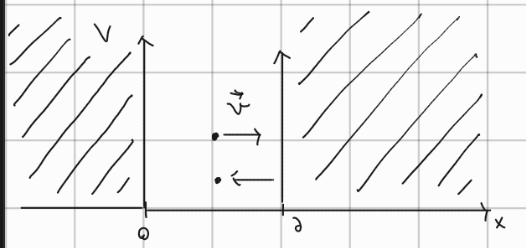
\includegraphics[width=\linewidth]{immagini/2026-04-09-16-43-51.png}
    \end{minipage}\hfill
    \begin{minipage}{0.65\textwidth}
        Consideriamo una particella di massa $m$ vincolata a muoversi in una regione unidimensionale di lunghezza $a$. L'energia potenziale è definita come: %
        \begin{equation}
            V(x) = \begin{cases}
                0 & \text{se } 0 \le x \le a \\ %
                \infty & \text{altrove (fuori dalla buca)} %
            \end{cases}
        \end{equation}
    \end{minipage}
\end{figure}

Risolviamo l'equazione di Schrödinger indipendente dal tempo: %
\begin{equation*}
    -\frac{\hbar^2}{2m} \frac{\partial^2 u}{\partial x^2} + V u = E u %
\end{equation*}

\noindent
\textbf{1. Fuori dalla buca ($x < 0$ e $x > a$):} %
Qui $V \to \infty$. Affinché l'energia totale $E$ rimanga una quantità fisica finita (e non diverga all'infinito), la funzione d'onda deve necessariamente annullarsi. %
\begin{equation*}
    u(x) = 0 \quad \text{per } x < 0 \text{ e } x > a %
\end{equation*}

\noindent
\textbf{2. Condizioni di Continuità ai bordi:} %
Poiché la funzione d'onda $\Psi$ deve essere ovunque continua (Proprietà 3), i limiti ai bordi della buca devono raccordarsi con lo zero esterno: %
\begin{equation}
    u(x=0) = 0 \quad \text{e} \quad u(x=a) = 0 \quad \text{(\textbf{Condizioni al contorno})} %
\end{equation}

\subsection{Soluzione all'interno della Buca ($0 \le x \le a$)} %

Dentro la buca $V=0$, quindi il sistema è identico a quello della particella libera: %
\begin{equation*}
    E = \frac{\hbar^2 k^2}{2m} \quad \Rightarrow \quad k^2 = \frac{2mE}{\hbar^2} \quad \Rightarrow \quad u(x) = A\cos(kx) + B\sin(kx) %
\end{equation*}

Applichiamo ora le condizioni al contorno per trovare le costanti $A$ e $B$: %
\begin{itemize}
    \item \textbf{Condizione in $\mathbf{x=0}$:} %
    \begin{equation*}
        u(0) = A\cos(0) + B\sin(0) = A \cdot 1 + 0 = 0 \quad \Rightarrow \quad \boxed{ A = 0 } %
    \end{equation*}
    La soluzione si riduce alla sola parte sinusoidale: $u(x) = B\sin(kx)$. %

    \item \textbf{Condizione in $\mathbf{x=a}$:} %
    \begin{equation*}
        u(a) = B\sin(ka) = 0 %
    \end{equation*}
    Scartiamo la soluzione banale $B=0$ (altrimenti non ci sarebbe nessuna particella). Affinché il seno si annulli, l'argomento deve essere un multiplo intero di $\pi$: %
    \begin{equation}
        ka = n\pi \quad \Rightarrow \quad \boxed{ k_n = \frac{n\pi}{a} } \quad \text{con } n = 1, 2, 3 \dots %
    \end{equation}
    \textit{($n=0$ si scarta perché darebbe $k=0 \Rightarrow u(x)=0$, annullando di nuovo la particella).}
\end{itemize}

\noindent
\textbf{Conseguenza FONDAMENTALE:} %
Confinando la particella, il vettore d'onda $k$ non può più assumere valori continui, ma è \textbf{QUANTIZZATO}. Sostituendo $k_n$ nell'espressione dell'energia, otteniamo uno \textbf{Spettro Discreto}: %
\begin{equation}
    \boxed{ E_n = \frac{\hbar^2 k_n^2}{2m} = \frac{\hbar^2 \pi^2 n^2}{2 m a^2} } \quad \text{(Autovalori dell'Energia)} %
\end{equation}

\subsection{Normalizzazione e Autofunzioni} %

Le autofunzioni spaziali, dipendenti dal \textbf{numero quantico} $n$, sono: %
\begin{equation*}
    u_n(x) = B\sin(k_n x) = B\sin\left(\frac{n\pi x}{a}\right) %
\end{equation*}

\noindent
Troviamo l'ampiezza $B$ imponendo la condizione di normalizzazione totale sulla probabilità: %
\begin{equation*}
    \int_0^a |\Psi|^2 \, dx = 1 \quad \Rightarrow \quad \int_0^a |B|^2 \sin^2\left(\frac{n\pi x}{a}\right) \, dx = 1 %
\end{equation*}
L'integrale del seno al quadrato su un numero intero di semiperiodi restituisce metà dell'intervallo ($a/2$). Quindi: %
\begin{equation*}
    |B|^2 \frac{a}{2} = 1 \quad \Rightarrow \quad \boxed{ B = \sqrt{\frac{2}{a}} } %
\end{equation*}

\begin{quote}
    \textbf{Soluzione Completa (Autovalori e Autofunzioni di $\hat{H}$):} %
    \begin{align}
        E_n &= \frac{\hbar^2 \pi^2}{2 m a^2} n^2 \\ %
        u_n(x) &= \sqrt{\frac{2}{a}} \sin\left(\frac{n\pi x}{a}\right) \quad \text{per } 0 \le x \le a %
    \end{align}
\end{quote}

\begin{figure}[H]
    \centering
    \begin{minipage}{0.3\textwidth}
        \centering
        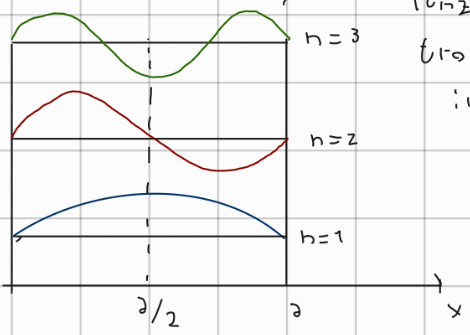
\includegraphics[width=\linewidth]{immagini/2026-04-09-16-51-23.png}
    \end{minipage}\hfill
    \begin{minipage}{0.7\textwidth}
        \textbf{Osservazioni Fisiche:} %
        \begin{itemize}
            \item I livelli di energia crescono con il quadrato del numero quantico ($E_n = n^2 E_1$). I livelli si distanziano sempre di più man mano che si sale. %
            \item Il livello fondamentale ($n=1$) \textbf{NON ha energia nulla} ($E_1 > 0$). Questo si chiama \textit{Energia di Punto Zero} ed è una conseguenza diretta del Principio di Indeterminazione di Heisenberg (se la particella fosse ferma con $E=0$, avrebbe $\Delta p = 0$, ma essendo confinata in $a$ ha un $\Delta x$ finito, il che violerebbe il principio). %
            \item Il modulo quadro di queste funzioni $|u_n(x)|^2$ fornisce la densità di probabilità di trovare la particella. Nello stato $n=2$, ad esempio, la probabilità di trovare la particella esattamente al centro della buca ($x=a/2$) è rigorosamente \textbf{ZERO} (nodo della funzione d'onda)! %
        \end{itemize}
    \end{minipage}
\end{figure}

\subsection{Proprietà Aggiuntive (Buca Infinita 1D)} %

\noindent
\textbf{1. Assenza dello stato $n=0$:} %
Il livello $n=0$ NON È PERMESSO. Se $n=0 \Rightarrow E=0$. La particella sarebbe ferma ($\Delta p = 0$). Tuttavia, l'incertezza sulla posizione $\Delta x$ vale al massimo $a$ (la larghezza della buca). Di conseguenza: %
\begin{equation*}
    \Delta x \Delta p = a \cdot 0 = 0 %
\end{equation*}
Questo violerebbe il Principio di Heisenberg. Deve quindi esistere un'Energia di punto zero $E_1 = \frac{\hbar^2 \pi^2}{2ma^2}$ %.

\noindent
\textbf{2. Parità delle Autofunzioni:} %
Rispetto al centro della buca ($x = a/2$), le funzioni d'onda hanno una PARITÀ ben definita: %
\begin{itemize}
    \item $n=1 \Rightarrow$ PARI (rispetto ad $a/2$) %
    \item $n=2 \Rightarrow$ DISPARI %
    \item $n=3 \Rightarrow$ PARI %
\end{itemize}
Regola aurea: $n$ dispari $\Rightarrow$ pari; $n$ pari $\Rightarrow$ dispari \textit{(Nota: se avessimo centrato la buca tra $-a/2$ e $a/2$, avremmo ottenuto direttamente seni per i dispari e coseni per i pari)} %.

\noindent
\textbf{3. Nodi e Ortogonalità:} %
Se il numero quantico $n$ aumenta, aumenta anche il numero di nodi (punti in cui $\Psi=0$) all'interno della buca.

\begin{enumerate}
    \setcounter{enumi}{3}
    \item \textbf{Ortogonalità:} Le autofunzioni formano una base ortonormale, verificabile tramite l'integrale del loro prodotto:
    \begin{equation}
        \int_0^a \sqrt{\frac{2}{a}} \sin\left(\frac{n\pi x}{a}\right) \cdot \sqrt{\frac{2}{a}} \sin\left(\frac{m\pi x}{a}\right) dx = \delta_{n,m} \quad \Rightarrow \quad \text{ortogonali}
    \end{equation}

    \item \textbf{Stato Generico e Probabilità:} Una qualsiasi funzione d'onda $\Psi(x)$ nella buca può essere scritta come serie delle autofunzioni:
    \begin{equation*}
        \Psi(x) = \sum_n c_n u_n(x) = \sqrt{\frac{2}{a}} \sum_n c_n \sin\left(\frac{n\pi x}{a}\right)
    \end{equation*}
    Calcoliamo i coefficienti $c_n$ proiettando la funzione $\Psi$ sull'autostato ennesimo:
    \begin{equation*}
        c_n = \int_0^a u_n^*(x) \Psi(x) \, dx = \sqrt{\frac{2}{a}} \int_0^a \sin\left(\frac{n\pi x}{a}\right) \Psi(x) \, dx
    \end{equation*}
    Per il postulato della misura, il modulo quadro del coefficiente è la probabilità di misurare quell'energia, e la loro somma deve fare $1$:
    \begin{equation*}
        |c_n|^2 = \mathbb{P}(E = E_n) \quad \Rightarrow \quad \sum_n |c_n|^2 = 1
    \end{equation*}

    \item \textbf{Cambio degli Estremi:} Se CAMBIO gli ESTREMI della buca (es. spostando l'origine al centro), la forma matematica delle $u_n(x)$ cambia.
    Le nuove condizioni al contorno impongono che la funzione si annulli sui nuovi bordi:
    \begin{equation*}
        u\left(x = \pm \frac{a}{2}\right) = 0
    \end{equation*}
    \textit{(Questo porterà ad avere seni per gli stati dispari e coseni per gli stati pari).}

    \item \textbf{Evoluzione Temporale Completa:} Unendo la parte spaziale e il fattore di fase temporale, la soluzione generale tempo-dipendente è:
    \begin{equation}
        \Psi(x,t) = \sum_n c_n \sqrt{\frac{2}{a}} \sin\left(\frac{n\pi x}{a}\right) e^{-i\frac{E_n}{\hbar}t}
    \end{equation}

    \item \textbf{Valore Medio del Momento:}
    \begin{equation}
        \langle \hat{p} \rangle = 0 \quad \Rightarrow \quad \text{Autostati REALI, in media la } v \text{ è } 0
    \end{equation}
    \textit{(Essendo la particella confinata, rimbalza continuamente a destra e sinistra, annullando la velocità vettoriale media).}
\end{enumerate}

\noindent
\textbf{9. Raccordo con il Limite Classico} %

\noindent
Classicamente, la probabilità di trovare una particella che rimbalza in una scatola è inversamente proporzionale alla sua velocità. Il tempo $dt$ speso tra $x$ e $x+dx$ è $dt = \frac{dx}{v}$: %
\begin{equation*}
    P_{class}(x \div x+dx) \propto dt \quad \Rightarrow \quad P_{class} \propto \frac{1}{v} %
\end{equation*}
Essendo l'energia cinetica $E_k$ fissata (conservazione dell'energia in una buca ideale), $v$ è costante, e quindi la probabilità classica è uniforme in tutta la buca: $P_{class} = \frac{1}{a} = \text{costante}$ %.

\begin{figure}[H]
    \centering
    \begin{minipage}{0.3\textwidth}
        \centering
        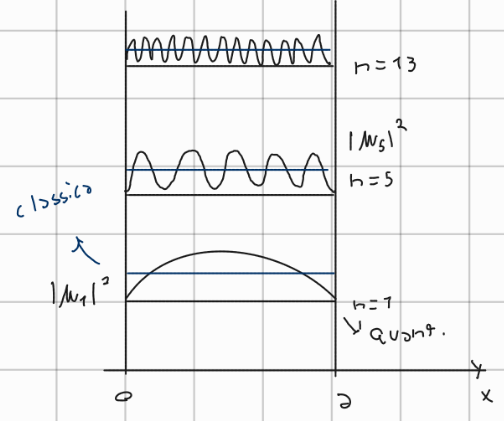
\includegraphics[width=\linewidth]{immagini/2026-04-09-17-00-22.png}
    \end{minipage}\hfill
    \begin{minipage}{0.65\textwidth}
        Quantisticamente, la probabilità per $n=1$ è una gobba al centro. Per $n=5$ sono cinque gobbe %. 
        \textbf{Principio di Corrispondenza:} Più $n$ cresce, più la funzione d'onda oscilla velocemente. Al limite di $n$ grandissimo, le infinite piccole oscillazioni si "spalmano" e il valore medio quantistico tende esattamente al valore costante della probabilità classica %!
    \end{minipage}
\end{figure}

\noindent
\textbf{Macroscopico vs Microscopico:} %
Sia un corpuscolo macroscopico con $m = 10^{-14}$ kg e $v = 1$ mm/s in una scatola di $a = 10$ cm. La sua energia cinetica è $\sim 10^{-21}$ J %.
Calcolando il suo numero quantico da $E_n = \frac{\hbar^2 \pi^2 n^2}{2ma^2}$, troviamo che il sistema si trova in un numero quantico $n \simeq 10^{15}$ %. 

\noindent
\textbf{Spaziatura dei Livelli:} %
\begin{equation*}
    \delta E = E_{n+1} - E_n \simeq \frac{\hbar^2 \pi^2}{2ma^2} [(n+1)^2 - n^2] \simeq \frac{\hbar^2 \pi^2}{2ma^2} 2n \quad \Rightarrow \quad \delta E \propto n %
\end{equation*}
Tuttavia, l'errore relativo $\frac{\delta E}{E} \propto \frac{n}{n^2} = \frac{1}{n}$ %.
Per $n \simeq 10^{15}$, l'errore relativo tende a zero. Lo spettro diventa per tutti gli scopi pratici \textbf{CONTINUO}, permettendoci di definire una "Densità degli Stati" $D(k)$: %
\begin{figure}[H]
    \centering
    \begin{minipage}{0.3\textwidth}
        \centering
        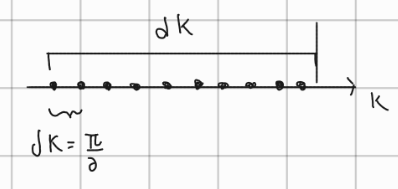
\includegraphics[width=\linewidth]{immagini/2026-04-09-17-01-32.png}
    \end{minipage}\hfill
    \begin{minipage}{0.65\textwidth}
        \begin{equation*}
            \Delta k = \frac{\pi}{a} \quad \Rightarrow \quad D(k) \, dk = \frac{dk}{\pi/a} = \frac{a}{\pi} dk \quad 
            \text{(\# stati compresi tra } k \text{ e } k+dk \text{)} %
        \end{equation*}
    \end{minipage}
\end{figure}

\section{Particella Confinata su un Anello (Rotore Rigido 1D)} %

\begin{figure}[H]
    \centering
    \begin{minipage}{0.3\textwidth}
        \centering
        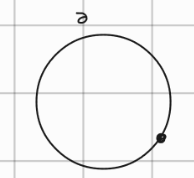
\includegraphics[width=\linewidth]{immagini/2026-04-09-17-16-57.png}
    \end{minipage}\hfill
    \begin{minipage}{0.65\textwidth}
        Studiamo una particella di massa $m$ libera di muoversi ma vincolata a una circonferenza di lunghezza totale $a = 2\pi R$ %.
        L'equazione di Schrödinger lungo la coordinata $x$ (srotolata sull'anello) è formalmente quella della particella libera: %
        \begin{equation*}
            -\frac{\hbar^2}{2m} \frac{d^2 u}{dx^2} = Eu \quad \Rightarrow \quad u(x) = A e^{ikx} %
        \end{equation*}
    \end{minipage}
\end{figure}

A differenza della buca, qui non ci sono pareti dove la funzione si annulla. Tuttavia, \textbf{il punto $x$ e il punto $x+a$ coincidono fisicamente} %.
Imponiamo le \textbf{Condizioni al Contorno CICLICHE} (o di periodicità): %
\begin{equation*}
    u(x+a) = u(x) %
\end{equation*}
Sostituendo l'esponenziale: %
\begin{equation*}
    A e^{ik(x+a)} = A e^{ikx} \quad \Rightarrow \quad e^{ikx} e^{ika} = e^{ikx} \quad \Rightarrow \quad e^{ika} = 1 %
\end{equation*}
Affinché $e^{ika} = 1$, l'argomento deve essere un multiplo intero di $2\pi$: %
\begin{equation}
    k a = 2n\pi \quad \Rightarrow \quad \boxed{ k_n = \frac{2\pi n}{a} } \quad \text{con } n = 0, \pm 1, \pm 2, \dots %
\end{equation}
(La quantizzazione nasce dalla topologia dello spazio!)

L'energia per la particella sull'anello è quindi quantizzata: %
\begin{equation}
    \boxed{ E_n = \frac{\hbar^2 k_n^2}{2m} = \frac{4 \hbar^2 \pi^2 n^2}{2 m a^2} = \frac{2 \hbar^2 \pi^2}{m a^2} n^2 } %
\end{equation}

Troviamo la costante di normalizzazione $A$: %
\begin{equation*}
    \int_0^a |A e^{ikx}|^2 dx = 1 \quad \Rightarrow \quad |A|^2 a = 1 \quad \Rightarrow \quad A = \frac{1}{\sqrt{a}} %
\end{equation*}

\noindent
\textbf{Spettro Energetico e Degenerazione:} %
\begin{itemize}
    \item $n = 0 \Rightarrow u_0(x) = \frac{1}{\sqrt{a}}$ e $E_0 = 0$. Lo stato fondamentale ha energia nulla ed è \textbf{NON degenere} (il principio di Heisenberg qui è salvo perché se $\Delta p = 0$, la posizione è totalmente incerta su tutto l'anello, $\Delta x \to \infty$ virtualmente sul cerchio) %.
    \item $n = \pm 1 \Rightarrow E_1 = \frac{2 \hbar^2 \pi^2}{m a^2}$. Le funzioni d'onda sono $u_1 = \frac{1}{\sqrt{a}} e^{i\frac{2\pi}{a}x}$ e $u_{-1} = \frac{1}{\sqrt{a}} e^{-i\frac{2\pi}{a}x}$. Corrispondono a rotazioni in sensi opposti (momento angolare destro e sinistro) e condividono la stessa energia $\Rightarrow$ Livello \textbf{2 volte DEGENERE} %.
\end{itemize}

% --- FINE BLOCCO ---


\end{document}